\chapter{分组并行求解算法及其应用}\label{ch03}
在微分方程的求解中, 许多方法最终都能归结于代数方程组的求解. 这些求解方法的主要困难在于最终的代数方程组规模过大, 无法在有限的时间内求解. 为了解决这个问题, 本文首先提出了一种分组并行的求解算法, 并将其实现为 PGSolve 软件包. 然后, 本文以求$n$-孤子和1-LUMP相互作用解的直接代数方法为例, 展示了 PGSolve 对于大规模代数方程组的求解能力. 

\section{分组并行求解算法与PGSolve软件包}
代数方程组的求解是符号计算的核心问题之一. 尤其是多项式代数方程组的求解, 更是符号计算中最基础也是最困难的问题. 多项式代数方程组的求解算法有吴文俊先生的吴方法\cite{wu1984,wu1985}\D 正则列方法\cite{kalkbrener1991three,lu1994searching}和\Grobner{}基方法\cite{adams1994introduction}等. 吴方法的实现有王东明的charsets\cite{wang1995implementation}等. 正则列方法的实现有 RegularChains \cite{maza2000triangular}, 该软件包已经被包含在 Maple 的内置函数中. 求\Grobner{}基的相关算法有 Buchberger 算法\cite{buchberger1970algorithmic}\D F4 算法\cite{faugere1999new} 和 F5 算法\cite{faugere2002new}等. Maple 和 Mathematica 等计算机代数系统的内置求解函数都是以\Grobner{}基方法为基础实现的, 且\Grobner{}基方法不仅能够求解多项式方程组, 还能求解更加一般的代数方程组. 

上述方法的基本原理是将原方程组转化一个或多个三角化的方程组后在逐个求解, 且三角化后的方程组和原方程同解. 但是, 算法关于方程规模的时间复杂度都是指数的, 并且计算过程中表达式的中间结果膨胀十分严重, 难以在有限的时间和内存条件下求解大规模的方程组. 并且, 上述算法注重数学上的严谨性, 致力于求解原方程组所有的解. 然而在实际求解过程中, 我们往往只需要一部分的解, 这些算法解的完整性反而成为了降低求解效率的重要原因. 

因此, 为了高效地从大规模的代数方程组解的用户想要的解, 本文基于如下几点想法, 提出了一个分组并行的代数方程组求解算法.
\begin{compactenum}[(1)]
\item 对原方程组进行合理的分组后依次求解, 完成一个分组的求解后, 将解代入剩余的方程中继续求解. 
\item 在求解过程中删除不满足用户要求的解, 以减少解的分支, 提高求解效率.
\item 在适当的步骤中采用并行策略进行加速, 充分利用多核计算机的性能.
\end{compactenum}

\subsection{核心框架}
\begin{figure}[htbp]
\centering 
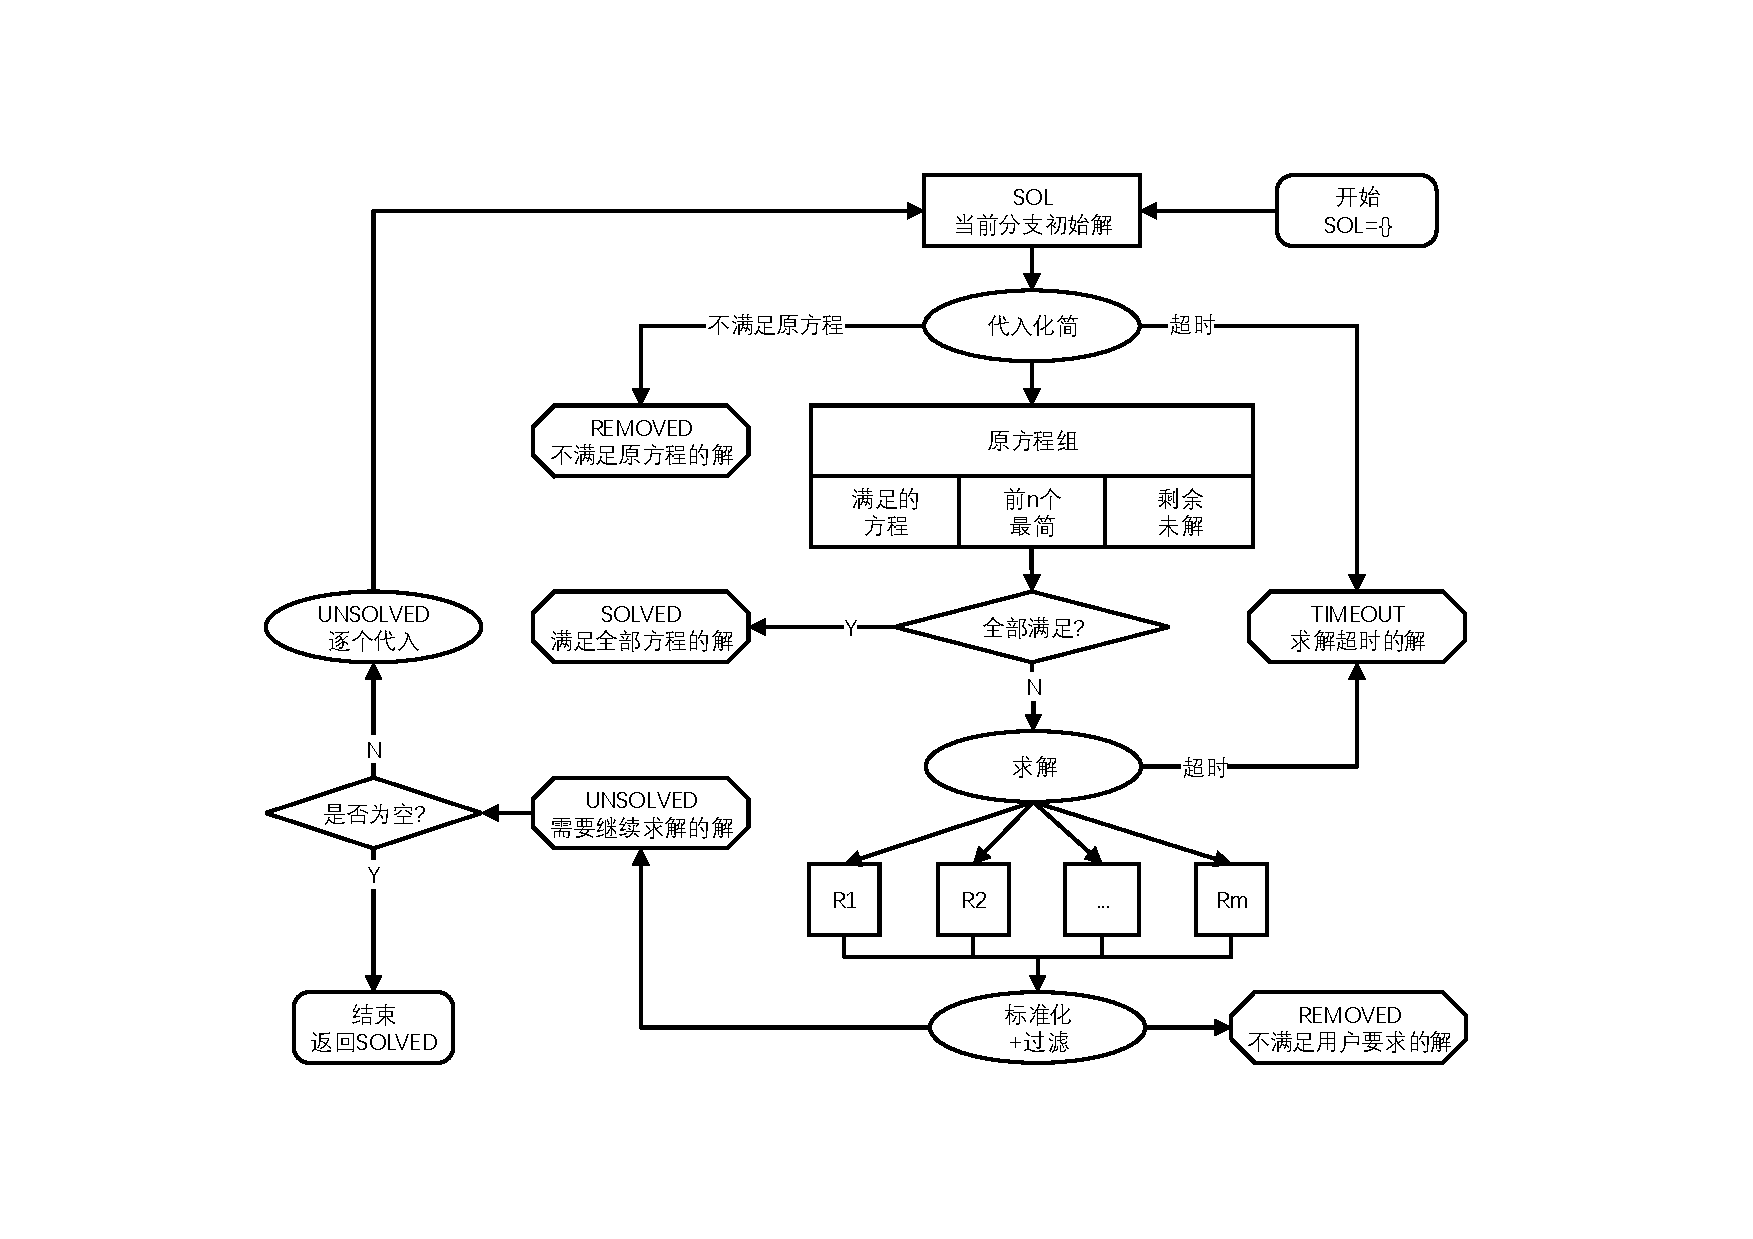
\includegraphics[width=0.9\textwidth]{fig/pgsolve.pdf}
\caption{PGSolve 算法框架}\label{PGSolve}
\end{figure}

根据上文的讨论, 本文设计如\reffig{PGSolve}所示的算法框架. 该算法的具体步骤如下:
\begin{compactenum}[Step 1.]
\item 初始化: 用于保存解集的 SOLVED\D UNSOLVED 以及 TIMEOUT 三个容器为空集. 令 SOL=\{\}. 
\item 将当前解SOL代入原方程组之后并化简. 化简之后, 原方程组可以分为三个部分. 第一部分是已经满足的方程, 这些方程在代入化简后为零. 将剩余的方程按照复杂度进行升序排序之后, 可以根据用户给定的n分为两个部分. 
\item 在代入化简后, 
    \begin{compactenum}[(a)]
    \item 如果存在一些方程的化简结果为常数, 则表示SOL不满足原方程组, 我们将其废弃后进入下一个分支的求解. 
    \item 若SOL满足原方程组的所有方程, 则将 SOL 加入 SOLVED之后继续下一个分支的求解. 
    \item 若化简超时, 则将 SOL 加入 TIMEOUT 后继续下一个分支的求解. 
    \item 否则, 就取尚未求解的方程中最简单的n个进行求解.
    \end{compactenum}
\item 若求解超时, 则将 SOL 加入 TIMEOUT. 否则, 就对求得的解进行标准化. 标准化包含以下几个步骤:
    \begin{compactenum}[(1)]
    \item 删除每个解中的自由变量. 这是因为 Maple 的 solve 在求解时会返回自由变量(如 x=x).
    \item res 中的每个解并上 sol 构成一个新的方程, 再利用 solve 进行求解, 保证解的最简性和唯一性. 
    \item 再次删除自由变量.
    \item 按照用户指定条件对解进行过滤, 删除不满足用户指定条件的解. 
    \end{compactenum}
\item 标准化之后, 按照用户给定的条件对解进行过滤, 将满足条件的解加入 UNSOLVED 继续求解. 
\item 如果此时 UNSOLVED 为空, 则算法结束, SOLVED 中包含了用户想要的解. 否则, 就将 UNSOLVED 内的元素全部取出之后, 依次作为 SOL 转 Step 2. 
\end{compactenum}


在上述算法中, 我们对代入化简后的方程组按照复杂度升序进行排序. 其目的在于降低求解的前n个方程所构成的方程组的复杂度.  因为要想利用分组策略提高方程组的求解效率, 就需要满足以下两个条件: (1) 前面的分组尽可能的简单, 减少单步的求解时间; (2) 前面的分组解的解尽可能的少, 以减小求解的分支数量. 

一个方程组的复杂度是由三个个方面决定的: 一方面是方程的数量, 方程的数量越多方程组就越复杂; 另一方面是方程组中变量的个数, 变量的个数越多方程组越复杂; 还有一方面是方程组中表达式的复杂度, 单个表达式长度越长, 次数越高, 则这个表达式越复杂. 出于这些考虑, 按复杂度排序的逻辑如下:
\begin{compactenum}[(1)]
\item 将方程按照变量进行分组, 变量相同的方程放在同一组内.
\item 将上述分组按照变量数量升序排序.
\item 每个分组内利用 Maple 的 \texttt{SolveTools:-Complexity} 函数衡量表达式的复杂度, 按照复杂度升序排序.  
\item 上述操作完成后, 将各个分组展开, 把方程组还原为一个列表. 
\end{compactenum}

按照上述策略进行排序就能保证所求解的前n个方程构成的方程组是最简的. 接着, 我们就要尽可能地控制解的数量以减少分支的数量. 在变量数目不变的情况下, 一个方程组解的数量和方程的数量相关. 一般而言, 方程数量越多, 约束约苛刻, 则解的数量就越少. 但是方程数量越多, 则求解这个方程组所需要的时间越长. 因此, 求解方程的数量是一个需要权衡的数字, 可以由用户根据实际情况进行设置, 而本文一般取 $n=5$.

此外需要特别说明的是, 我们将SOL代入所有的方程进行代入化简的主要原因如下: 
\begin{compactenum}[(1)]
\item 对尚未求解的方程进行代入化简, 能够对新的方程组按照复杂度重新排序, 从而获得更简单的方程.
\item 对已经求解过的方程进行代入化简, 能够验证当前分支的解是否满足这部分方程. 
\item 以便在获得原方程的解时直接返回. 此时, 尽管我们只求解了部分方程, 但是求得的解能够全部方程时, 就能提起阶数分支, 将当前的解添加到 SOLVED 中. 
\end{compactenum} 

而在 TIMEOUT 中保存超时的解的意义在于, 如果用户可以在求解结束时愿意花更多的时间来继续求解超时的解, 就将 TIMEOUT 复制给 UNSOLVED 之后, 设定更大的时限重新求解. 

\subsection{并行调度策略} 
在\reffig{PGSolve}所示的算法中, 除了``求解''以外的三个椭圆形节点所代表的步骤都能够并行化. 在实际求解过程中, 
\begin{compactitem}[*]
\item ``代入化简''所需的时间最长, 而化简一个表达是又是一个工作量比较小的原子任务, 比较适合对其进行并行化.
\item ``标准化+过滤''所需的时间极短, 进行并行加速的意义不大.
\item ``UNSOLVED逐个代入''这个步骤的每个子任务所包含的工作量过大, 不适合并行加速.
\end{compactitem}
因此, 我们选择将``代入化简''这一步并行化. 而我们所采用的并行调度策略是经典的Master-Slave调度模型\cite{sahni1996master}. 

如\reffig{msp}所示, Master-Slave 调度模型的原理如下:
\begin{compactenum}[Step 1.]
\item 所有并行任务进入任务池.
\item Master 节点从任务池拉取任务分配给空闲的 Slave 节点, 直到没有空闲节点.
\item Slave 完成任务后返回, Master 将新的任务分配给当前 Slave 节点, 直至所有任务完成. 
\end{compactenum}

\begin{figure}[htbp]
\centering 
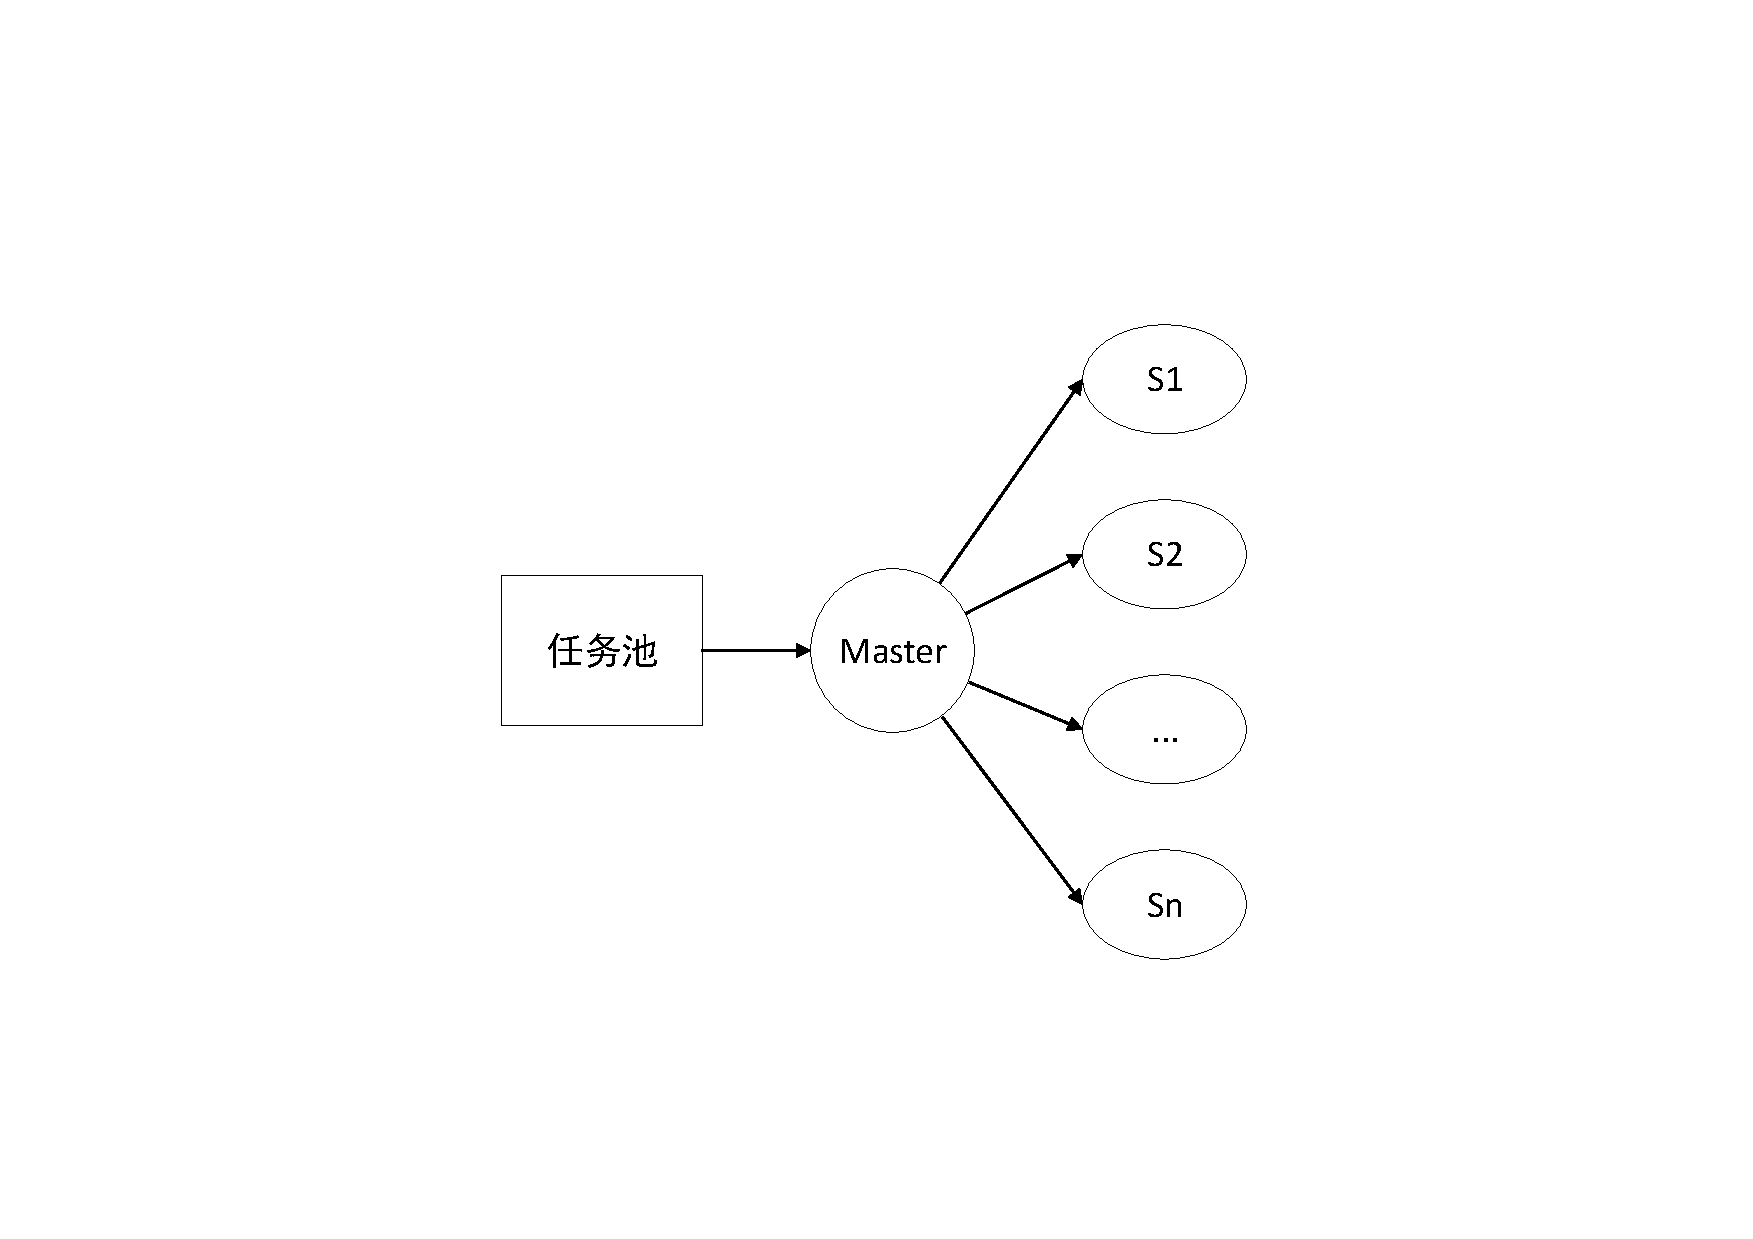
\includegraphics[width=0.8\textwidth]{fig/msp.pdf}
\caption{Master-Slave 调度模型}\label{msp}
\end{figure}

\subsection{PGSolve软件包的接口与实现}

\section{PGSolve在直接代数方法中的应用}
\section{小结}
